% Copyright 2005 by Till Tantau <tantau@cs.tu-berlin.de>.
%
% This program can be redistributed and/or modified under the terms
% of the LaTeX Project Public License Distributed from CTAN
% archives in directory macros/latex/base/lppl.txt.


\section{Syntax for Path Specifications}

A \emph{path} is a series of straight and curved line segments. It is
specified following a |\path| command and the specification must
follow a special syntax, which is described in the subsections of the
present section.


\begin{command}{\path\meta{specification}|;|}
  This command is available only inside a |{tikzpicture}| environment
  and  only if the \tikzname\ package is loaded.

  The \meta{specification} is a long stream of \emph{path
  operations}. Most of these path operations tell \tikzname\ how the path
  is build. For example, when you write |--(0,0)|, you use a
  \emph{lineto operation} and it means ``continue the path from
  wherever you are to the origin.''

  At any point where \tikzname\ expects a path operation, you can also
  give some graphic options, which is a list of options in brackets,
  such as |[rounded cornders]|. These options can have different
  effects:
  \begin{enumerate}
  \item
    Some options take ``immediate'' effect and apply to all subsequent
    path operations on the path. For example, the |rounded corners|
    option will round all following corners, but not the corners
    ``before'' and if the |sharp corners| is given later on the path
    (in a new set of brackets), the rounding effect will end.

\begin{codeexample}[]
\tikz \draw (0,0) -- (1,1)
           [rounded corners] -- (2,0) -- (3,1)
           [sharp corners] -- (3,0) -- (2,1);
\end{codeexample}
    Another example are the transformation options, which also apply
    only to subsequent coordinates.
  \item
    The options that have immediate effect can be ``scoped'' by
    putting part of a path in curly braces. For example, the above
    example could also be written as follows:

\begin{codeexample}[]
\tikz \draw (0,0) -- (1,1)
           {[rounded corners] -- (2,0) -- (3,1)}
           -- (3,0) -- (2,1);
\end{codeexample}
  \item
    Some options only apply to the path as a whole. For example, the
    |color=| option for determining the color used for, say, drawing
    the path always applies to all parts of the path. If several
    different colors are given for different parts of the path, only
    the last one (on the outermost scope) ``wins'':
 
\begin{codeexample}[]
\tikz \draw (0,0) -- (1,1)
           [color=red] -- (2,0) -- (3,1)
           [color=blue] -- (3,0) -- (2,1);
\end{codeexample}

    Most options are of this type. In the above example, we would have
    had to ``split up'' the path into several |\path| commands:
\begin{codeexample}[]
\tikz{\draw (0,0) -- (1,1);
      \draw [color=red] (2,0) -- (3,1);
      \draw [color=blue] (3,0) -- (2,1);}
\end{codeexample}
  \end{enumerate}

  By default, the |\path| command does ``nothing'' with the
  path, it just ``throws it away.'' Thus, if you write
  |\path(0,0)--(1,1);|, nothing is drawn 
  in your picture. The only effect is that the area occupied by the
  picture is (possibly) enlarged so that the path fits inside the
  area. To actuall ``do'' something with the path, an option like
  |draw| or |fill| must be given somewhere on the path. Commands like
  |\draw| do this implicitly.
  
  Finally, it is also possible to give \emph{node specifications} on a
  path. Such specifications can come at different locations, but they
  are always allowed when a normal path operation could follow. A node
  specification starts with |node|. Basically, the effect is to
  typeset the node's text as normal \TeX\ text and to place
  it at the ``current location'' on the path. The details are exlained
  in Section~\ref{section-nodes}.

  Note, however, that the nodes are \emph{not} part of the path in any
  way. Rather, after everything has been done with the path what is
  specified by the path options (like filling and drawing the path due
  to a |fill| and a |draw| option somewhere in the
  \meta{specification}), the nodes are added in a post-processing
  step.   
  
  The following style influences scopes:
  \begin{itemize}
    \itemstyle{every path}
    This style is installed at the beginning of every path. This can
    be useful for (temporarily) adding, say, the |draw| option to
    everything in a scope.
\begin{codeexample}[]

\begin{tikzpicture}[fill=yellow!50!black] % only sets the color
  \tikzstyle{every path}=[draw]           % all paths are drawn
  \fill  (0,0) rectangle +(1,1);
  \shade (2,0) rectangle +(1,1);
\end{tikzpicture}
\end{codeexample}
  \end{itemize}
\end{command}




\subsection{The Move-To Operation}

A \emph{move-to operation} normally starts a path at a certain
point. This does not cause a line segment to be created, but it
specifies the starting point of the next segment. If a path is
already under construction, that is, if several segments have
already been created, a move-to operation will start a new part of the
path that is not connected to any of the previous segments.

The syntax for specifying a move-to operation is easy:
\declare{\meta{coordinate}}. Simply provide a coordinate in round
brackets. For example, the following command (when used inside a
|{tikzpicture}| environment) draws two lines: 

\begin{codeexample}[]
\begin{tikzpicture}
  \draw (0,0) --(2,0) (0,1) --(2,1);
\end{tikzpicture}
\end{codeexample}

In the specification |(0,0) --(2,0) (0,1) --(2,1)| two move-to
operations are specified: |(0,0)| and |(0,1)|. The other two
operations, namely |--(2,0)| and |--(2,1)| are line-to operations,
described next.


\subsection{The Line-To Operation}

A \emph{line-to operation} extends the current path from the current
point in a straight line to the given coordinate. The ``current
point'' is the endpoint of the previous drawing command or the point
specified by a prior moveto operation.

Syntax of the line-to operation: \declare{|--|\meta{coordinate}}. You
use two minus signs followed by a coordinate in round brackets. You
can add spaces before and after the~|--|.

When a line-to operation is used and some path segment has just been
constructed, for example by another line-to operation, the two line
segments become joined. This means that if they are drawn, the point
where they meet is ``joined'' smoothly. To appreciate the difference,
consider the following two examples: In the left example, the path
consists of two path segments that are not joined, but that happen to
share a point, while in the right example a smooth join is shown.

\begin{codeexample}[]

\begin{tikzpicture}[line width=10pt]
  \draw (0,0) --(1,1)  (1,1) --(2,0);
  \draw (3,0) -- (4,1) -- (5,0);
\end{tikzpicture}
\end{codeexample}



\subsection{Horizontal/Vertical Line-To Operations}

Sometimes you want to connect two points via straight lines that are
only horizontal and vertical. For this, you can use the path
construction commands \verb!-|! and \verb!|-!. The first means
``first horizontal, then vertical,'' the second means ``first
vertical, then horizontal.''

Syntax of these versions of the line-to operation:
\declare{\verb!-|!\meta{coordinate}} and
\declare{\verb!|-!\meta{coordinate}}. You can add spaces for clarity. 

Here is an example:

\begin{codeexample}[]
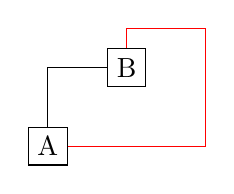
\begin{tikzpicture}
  \draw (0,0) node(a) [draw] {A}  (1,1) node(b) [draw] {B};
  \draw (a.north) |- (b.west);
  \draw[color=red] (a.east) -| (2,1.5) -| (b.north);
\end{tikzpicture}
\end{codeexample}


\subsection{The Curveto Operation}

A \emph{curveto operation} extends the current path from the current
point, let us call it $x$, via a curve to a new current point, let us
call it $y$. The curve is a so-called Bezi�r curve. For such a curve,
apart from $y$, you also specify two control points $c$ and $d$. The
idea is that the curve starts at $x$, ``heading'' in the direction
of~$c$. Mathematically spoken, the tangent of the curve at $x$ goes
through $c$. Similarly, the curve ends at $y$, ``coming from'' the
other control point,~$d$. The larger the distance between $x$ and~$c$
and between $d$ and~$y$, the larger the curve will be.

Syntax of the line-to operation:
\declare{|..controls|\meta{c}}\opt{|and|\meta{d}}\declare{|..|\meta{y}}. If
\meta{d} is not given, $d$ is assumed to be equal to $c$. 

\begin{codeexample}[]
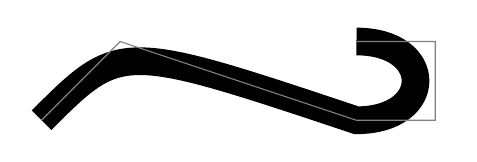
\begin{tikzpicture}
  \draw[line width=10pt] (0,0) .. controls (1,1) .. (4,0)
                               .. controls (5,0) and (5,1) .. (4,1);
  \draw[color=gray] (0,0) -- (1,1) -- (4,0) -- (5,0) -- (5,1) -- (4,1);
\end{tikzpicture}
\end{codeexample}

As with the line-to operation, it makes a difference whether two curves
are joined because they resulted from consecutive curve-to or line-to
operations, or whether they just happen to have the same ending:

\begin{codeexample}[]

\begin{tikzpicture}[line width=10pt]
  \draw (0,0) -- (1,1) (1,1) .. controls (1,0) and (2,0) .. (2,0);
  \draw (3,0) -- (4,1) .. controls (4,0) and (5,0) .. (5,0);
\end{tikzpicture}
\end{codeexample}


\subsection{The Cycle Operation}

A \emph{cycle operation} adds a straight line from the current
point to the last point specified by a move-to operation. Note that
this need not be the beginning of the path. Furthermore, a smooth join
is created between the first segment created after the last move-to
operation and the straight line appended by the cycle operation.

Syntax of the line-to operation:
\declare{|--cycle|}. You can add a space between |--| and |cycle| for
clarity.  

Consider the following example. In the left example, two triangles are
created using three straight lines, but they are not joined at the
ends. In the second example cycle operations are used.

\begin{codeexample}[]

\begin{tikzpicture}[line width=10pt]
  \draw (0,0) -- (1,1) -- (1,0) -- (0,0) (2,0) -- (3,1) -- (3,0) -- (2,0);
  \draw (5,0) -- (6,1) -- (6,0) -- cycle (7,0) -- (8,1) -- (8,0) -- cycle;
\end{tikzpicture}
\end{codeexample}


\subsection{Rounding Corners}

All of the path construction commands mentioned up to now are
influenced by the following option:
\begin{itemize}
  \itemoption{rounded corners}\opt{|=|\meta{inset}}
  When this option is in force, all corners (places where a line is
  continued either via line-to or a curve-to operation) are replaced by
  little arcs so that the corner becomes smooth. 

\begin{codeexample}[]
\tikz \draw [rounded corners] (0,0) -- (1,1)
           -- (2,0) .. controls (3,1) .. (4,0);
\end{codeexample}

  The \meta{inset} describes how big the corner is. Note that the
  \meta{inset} is \emph{not} scaled along if you use a scaling option
  like |scale=|. 

\begin{codeexample}[]
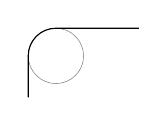
\begin{tikzpicture}
  \draw[color=gray,very thin] (10pt,15pt) circle (10pt);
  \draw[rounded corners=10pt] (0,0) -- (0pt,25pt) -- (40pt,25pt);
\end{tikzpicture}
\end{codeexample}

  You can switch the rounded corners on and off ``in the middle of
  path'' and different corners in the same path can have different
  corner radii:

\begin{codeexample}[]
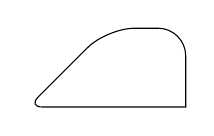
\begin{tikzpicture}
  \draw (0,0) [rounded corners=10pt] -- (1,1) -- (2,1)
                     [sharp corners] -- (2,0)
               [rounded corners=5pt] -- cycle;
\end{tikzpicture}
\end{codeexample}

\example Here is a rectangle with rounded corners:
\begin{codeexample}[]
\tikz \draw[rounded corners=1ex] (0,0) rectangle (20pt,2ex);
\end{codeexample}

  You should be aware, that there are several pitfalls when using this
  option. First, the rounded corner will only be an arc (part of a
  circle) if the angle is $90^\circ$. In other cases, the rounded
  corner will still be round, but ``not as nice.''

  Second, if there are very short line segements in a path, the
  ``rounding'' may cause inadverted effects. In such case it may be
  necessary to temporarily switch off the rounding using
  |sharp corners|. 

  \itemoption{sharp corners}
  This options switches off any rounding on subsequent corners of the
  path.   
\end{itemize}



\subsection{The Rectangle Operation}

A rectangle can obviously be created using four straight lines and a
cycle operation. However, since rectangles are needed so often, a
special syntax is available for them. When the rectangle operation is
used, one corner will be the current point, another corner will be
given by the specified point. The specified point becomes the new
current point.

Syntax of the rectanlge operation: \declare{|rectangle|\meta{corner}}. You
can add a space.

\begin{codeexample}[]
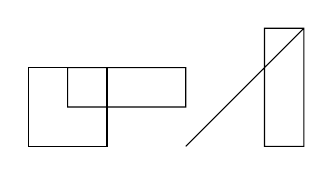
\begin{tikzpicture}
  \draw (0,0) rectangle (1,1);
  \draw (.5,1) rectangle (2,0.5) (3,0) rectangle (3.5,1.5) -- (2,0);
\end{tikzpicture}
\end{codeexample}


\subsection{The Circle and Ellipse Operations}

A circle can be approximated well using four Bezi�r curves. However,
it is difficult to do so correctly. For this reason, a special syntax
is available for adding such an approximation of a circle to the
current path. The center of the circle is given by the current
point. The new current point of the path will remain to be the center
of the circle. 

Syntax of the circle operation:
\declare{|circle(|\meta{radius}|)|}. You can add spaces.

Syntax of the ellipse operation:
\declare{|ellipse(|\meta{half width}| and |\meta{half height}|)|}. You
can add spaces after |ellipse| and you have to place spaces around |and|.  

\begin{codeexample}[]
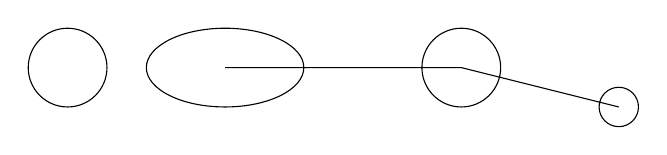
\begin{tikzpicture}
  \draw (1,0) circle (.5cm);
  \draw (3,0) ellipse (1cm and .5cm) -- ++(3,0) circle (.5cm)
    -- ++(2,-.5) circle (.25cm);
\end{tikzpicture}
\end{codeexample}


\subsection{The Arc Operation}

The \emph{arc operation} allows you to add an arc to the current
path. You provide a start angle, an end angle, and a radius. The arc
operation will then add a part of a circle of the given radius between
the given angles. The arc will start at the current point and will end
at the end of the arc.

Syntax for the arc operation: \declare{|arc(|\meta{start
    angle}|:|\meta{end
    angle}|:|\meta{radius}\opt{|/|\meta{half height}}|)|}.

\begin{codeexample}[]
\begin{tikzpicture}
  \draw (0,0) arc (180:90:1cm) -- (2,.5) arc (90:0:1cm);
  \draw (4,0) -- +(30:1cm) arc (30:60:1cm) -- cycle;
  \draw (8,0) arc (0:270:1cm/.5cm) -- cycle;
\end{tikzpicture}
\end{codeexample}

\begin{codeexample}[]
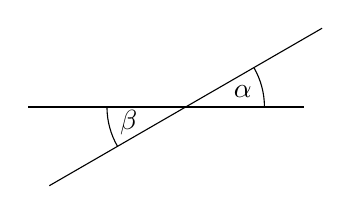
\begin{tikzpicture}
  \draw (-1,0) -- +(3.5,0);
  \draw (1,0) ++(210:2cm) -- +(30:4cm);
  \draw (1,0) +(0:1cm) arc (0:30:1cm);      
  \draw (1,0) +(180:1cm) arc (180:210:1cm);
  \path (1,0) ++(15:.75cm) node{$\alpha$};
  \path (1,0) ++(15:-.75cm) node{$\beta$};
\end{tikzpicture}
\end{codeexample}


\subsection{The Grid Operation}

You can add a grid to the current path using the |grid| path
operation. 

Syntax for the grid operation: \declare{|grid|\meta{corner
    coordinate}}.

The effect of the grid operation is the following: It will draw a grid
filling a rectangle whose two corners are given by \meta{corner
  coordinate} and by the previous coordinate. Thus, the typical way in
which a grid is drawn is |\draw (1,1) grid (3,3);|, which yields a
grid filling the rectangle whose corners are at $(1,1)$ and $(3,3)$.
All coordinate transformations apply to the grid.

\begin{codeexample}[]
\tikz[rotate=30] \draw[step=1mm] (0,0) grid (2,2);
\end{codeexample}

The stepping of the grid is governed by the following options:

\begin{itemize}
  \itemoption{step}|=|\meta{dimension} sets the stepping in both the
  $x$ and $y$-direction.
  \itemoption{xstep}|=|\meta{dimesion} sets the stepping in the
  $x$-direction. 
  \itemoption{ystep}|=|\meta{dimesion} sets the stepping in the
  $y$-direction. 
\end{itemize}

It is important to note that the grid is always ``phased'' such that
it contains the point $(0,0)$ if that point happens to be inside the
rectangle. Thus, the grid does \emph{not} always have an intersection
at the corner points; this occurs only if the corner points are
multiples of the stepping. Note that due to rounding errors, the
``last'' lines of a grid may be ommitted. In this case, you have to
add an epsilon to the corner points.

The following styles are useful for drawing grids:
\begin{itemize}
  \itemstyle{help lines}
  This style makes lines ``subdued''by using thin gray lines for
  them. However, this style is not installed automatically and you
  have to say for example:
\begin{codeexample}[]
\tikz \draw[style=help lines] (0,0) grid (3,3);
\end{codeexample}
\end{itemize}


\subsection{The Parabola Operation}

The |parabola| path command continues the current path with a
parabola. A parabola is a (shifted and scaled) curve defined by the
equation $f(x) = x^2$ and looks like this: \tikz \draw (-1ex,1.5ex)
parabola (1ex,0ex);.

The basic syntax of the parabola command is
\declare{|parabola|\meta{coordinate}}. This will draw a parabola that
``fills'' the rectangle whose corners are the old current point and
\meta{coordinate}. Here is an example:

\begin{codeexample}[]
\tikz \draw (0,0) rectangle (1,1)  (0,0) parabola (1,1);
\end{codeexample}

In detail, the parabola has the following properties: The old current
point lies in one corner of the rectangle and the parabola ``goes
through'' this point. The parabola will \emph{not} end at the given
\meta{coordinate}. Rather, it will have its bend on the 
$y$-coordinate of \meta{coordinate}. It will end on the $x$-coordinate
of \meta{coordinate} and the $y$-coordinate of the old current point.

Sometimes you may want to draw only a ``part'' of a parabola. For
this, you can  use |parabola left| and |parabola right|.

The syntax of the first command is
\declare{|parabola left|\meta{coordinate}}. This will draw the ``left
part'' of a parabola. More precisely, a parabola is drawn that goes
through the cold current point and has its bend at
\meta{coordinate}. Here is an example:
\tikz \draw (-1ex,1.5ex) parabola left (0,0);, which is obtained through the command
|\tikz \draw (-1ex,1.5ex) parabola left (0,0);|.

Similarly, there exists a \declare{|parabola right|\meta{coordinate}}
command. Here, the parabola has its bend at the old current point and
goes through the new \meta{coordinate}.

You can use |parabola left| and |parabola right| to draw parts of
parabolas. However, it is not possible to draw only a part of a
parabola that does not contain the bend. For this you need to use a
|plot| command.

\begin{codeexample}[]
\tikz \draw[scale=0.25] (-1,1) parabola left (0,0) parabola right (2,4);
\end{codeexample}

\begin{codeexample}[]
\tikz \draw[rotate=-90] (-1.5,2.25) node[right]{$\sqrt x$} parabola left(0,0);
\end{codeexample}

\subsection{The Sine and Cosine Operation}

The |sin| and |cos| operations are similar to the |parabola|
command. They, too, can be used to draw (parts of) a sine or cosine
curve.

Syntax: \declare{|sin|\meta{coordiante}} and
\declare{|cos|\meta{coordinate}}.

The effect of |sin| is to draw a scaled and shifted version of a sine
curve in the interval $[0,\pi/2]$. The scaling and shifting is done in
such a way that the start of the sine curve in the interval is at the
old current point and that the end of the curve in the interval is at
\meta{coordinate}. Here is an example that should clarify this:

\begin{codeexample}[]
\tikz \draw (0,0) rectangle (1,1)     (0,0) sin (1,1)
           (2,0) rectangle +(1.57,1) (2,0) sin +(1.57,1);
\end{codeexample}

The |cos| operation works similarly, only a cosine in the interval
$[0,\pi/2]$ is drawn. By correctly alternating |sin| and |cos|
operations, you can create a complete sine or cosine curve:

\begin{codeexample}[]
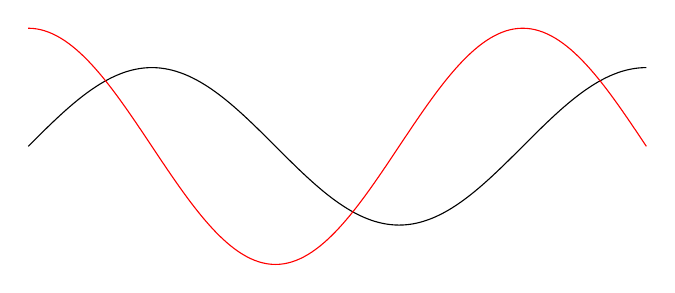
\begin{tikzpicture}[xscale=1.57]
  \draw (0,0) sin (1,1) cos (2,0) sin (3,-1) cos (4,0) sin (5,1);
  \draw[color=red] (0,1.5) cos (1,0) sin (2,-1.5) cos (3,0) sin (4,1.5) cos (5,0);
\end{tikzpicture}
\end{codeexample}


Note that there is no way to (conveniently) draw an interval on a sine
or cosine curve whose end points are not multiples of $\pi/2$ (or $90^\circ$).



\subsection{The Plot Operation}

The |plot| operation can be used to append a line or curve to the path
that goes through a large numbor of coordiantes. These coordinates are
either given in a simple list of coordinates or they are read from
some file.

The syntax of the |plot| comes in different versions. First, the
``beginning'' of a |plot| command can be
\begin{enumerate}
\item
  \declare{|plot|} or
\item
  \declare{|--plot|} (space may be added for clarity)
\end{enumerate}

The difference between the first and the second case is that |plot|
will start plotting at the first coordinate by ``moving'' to that
point. The |--plot| will instead perform a |--| (line-to) operation to
the first point of the plot.

Next, there are three ways of specifying the coordinates of the points
to be plotted:

\begin{enumerate}
\item
  \opt{|--|}|plot|\oarg{local options}\declare{|coordinates{|\meta{coordinate
    1}\meta{coordinate 2}\dots\meta{coordinate $n$}|}|}
\item
  \opt{|--|}|plot|\oarg{local options}\declare{|file{|\meta{filename}|}|}
\item
  \opt{|--|}|plot|\oarg{local options}\declare{|function{|\meta{gnuplot formula}|}|}
\end{enumerate}

These different ways are explained in the following.


\subsubsection{Plotting Points Given Inline}

In the first two cases, the points are given directly in the \TeX-file
as in the following example:

\begin{codeexample}[]
\tikz \draw plot coordinates {(0,0) (1,1) (2,0) (3,1) (2,1) (10:2cm)};
\end{codeexample}

Here is an example showing the difference between |plot| and |--plot|:

\begin{codeexample}[]
\begin{tikzpicture}
  \draw (0,0) -- (1,1) plot coordinates {(2,0)  (4,0)};
  \draw[color=red,xshift=5cm]
        (0,0) -- (1,1) -- plot coordinates {(2,0)  (4,0)};
\end{tikzpicture}
\end{codeexample}


\subsubsection{Plotting Points Read From an External File}

In the third and fourth form the points reside in an external
file named \meta{filename}. Currently, the only file format that
\tikzname\ allows is the following: Each line of the \meta{filename}
should contain one line starting with two numbers, separated by a
space. Anything following the two numbers on the line is
ignored. Also, lines starting with a |%| or a |#| are ignored as well
as empty lines. (This is exactly the format that \textsc{gnuplot}
produces when you say |set terminal table|.) If necessary, more
formats will be supported in the future, but it is usually easy to
produce a file containing data in this form.

\begin{codeexample}[]
\tikz \draw plot[mark=x,smooth] file {plots/pgfmanual-sine.table};
\end{codeexample}

The file |plots/pgfmanual-sine.table| reads:
\begin{codeexample}[code only]
#Curve 0, 20 points
#x y type
0.00000 0.00000  i
0.52632 0.50235  i
1.05263 0.86873  i
1.57895 0.99997  i
...
9.47368 -0.04889  i
10.00000 -0.54402  i
\end{codeexample}
It was produced from the following source, using |gnuplot|:
\begin{codeexample}[code only]
set terminal table
set output "../plots/pgfmanual-sine.table"
set format "%.5f"
set samples 20
plot [x=0:10] sin(x)
\end{codeexample}

The \meta{local options} of the |plot| command are local to each
plot and do not affect other plots ``on the same path.'' For example,
|plot[yshift=1cm]| will locally shift the plot 1cm upward. Remember,
however, that most options can only be applied to paths as a
whole. For example, |plot[red]| does not have the effect of making the
plot red. After all, you are trying to ``locally'' make part of the
path red, which is not possible.

\subsubsection{Plotting a Function}
\label{section-tikz-gnuplot}

Often, you will want to plot points that are given via a function like
$f(x) = x \sin x$. Unfortunately, \TeX\ does not really have enough
computational power to generate the points on such a function
efficiently (it is a text processing program, after all). However,
if you allow it, \TeX\ can try to call external programs that can
easily produce the necessary points. Currently, \pgfname\ knows how to
call \textsc{gnuplot}.

When \tikzname\ encounters your command
|plot[id=|\meta{id}|] function{x*sin(x)}| for 
the first time, it will create a file called
\meta{prefix}\meta{id}|.gnuplot|, where \meta{prefix} is |\jobname.| by
default, that is, the name of you main |.tex| file. If no \meta{id} is
given, it will be empty, which is allright, but it is better when each
plot has a unique \meta{id} for reasons explained in a moment. Next,
\tikzname\ writes some initialization code into this file followed by
|plot x*sin(x)|. The initialization code sets up things 
such that the |plot| command will write the coordinates into another
file called \meta{prefix}\meta{id}|.table|. Finally, this table file
is read as if you had said |plot file{|\meta{prefix}\meta{id}|.table}|. 

For the plotting mechansim to work, two conditions must be met:
\begin{enumerate}
\item
  You must have allowed \TeX\ to call external programs. This is often
  switched off by default since this is a securtiy risk (you might,
  without knowing, run a \TeX\ file that calls all sorts of ``bad''
  commands). To enable this ``calling external programs'' a command
  line option must be given to the \TeX\ program. Usually, it is
  called something like |shell-escape| or |enable-write18|. For
  example, for my |pdflatex| the option |--shell-escape| can be
  given.
\item
  You must have installed the |gnuplot| program and \TeX\ must find it
  when compiling your file.
\end{enumerate}

Unfortunately, these conditions will not always be met. Especially if
you pass some source to a coauthor and the coauthor does not have
\textsc{gnuplot} installed, he or she will have trouble compiling your
files.

For this reason, \tikzname\ behaves differently when you compile your
graphic for the second time: If upon reaching
|plot[id=|\meta{id}|] function{...}| the file \meta{prefix}\meta{id}|.table|
already exists \emph{and} if the \meta{prefix}\meta{id}|.gnuplot| file
contains what \tikzname\ thinks that it ``should'' contain, the |.table|
file is immediately read without trying to call a |gnuplot|
program. This approach has the following advantages: 
\begin{enumerate}
\item
  If you pass a bundle of your |.tex| file and all |.gnuplot| and
  |.table| files to someone else, that person can \TeX\ the |.tex|
  file without having to have |gnuplot| installed.
\item
  If the |\write18| feature is switched off for security reasons (a
  good idea), then, upon the first compilation of the |.tex| file, the
  |.gnuplot| will still be generated, but not the |.table|
  file. You can then simply call |gnuplot| ``by hand'' for each
  |.gnuplot| file, which will produce all necessary |.table| files.
\item
  If you change the function that you wish to plot or its
  domain, \tikzname\ will automatically try to regenerate the |.table|
  file.
\item
  If, out of laziness, you do not provide an |id|, the same |.gnuplot|
  will be used for different plots, but this is not a problem since
  the |.table| will automatically be regenerated for each plot
  on-the-fly. \emph{Note: If you intend to share your files with
  someone else, always use an id, so that the file can by typset
  without having \textsc{gnuplot} installed.} Also, having unique ids
  for each plot will improve compilation speed since no external
  programs need to be called, unless it is really necessary.
\end{enumerate}

When you use |plot function{|\meta{gnuplot formula}|}|, the \meta{gnuplot
  formula} must be given in the |gnuplot| syntax, whose details are
beyond the scope of this manual. Here is the ultra-condensed
essence: Use |x| as the variable and use the C-syntax for normal
plots, use |t| as the variable for parametric plots. Here are some examples:

\begin{codeexample}[]
\begin{tikzpicture}[domain=0:4]
  \draw[very thin,color=gray] (-0.1,-1.1) grid (3.9,3.9);
  
  \draw[->] (-0.2,0) -- (4.2,0) node[right] {$x$};
  \draw[->] (0,-1.2) -- (0,4.2) node[above] {$f(x)$};
  
  \draw[color=red]    plot[id=x]   function{x}           node[right] {$f(x) =x$};
  \draw[color=blue]   plot[id=sin] function{sin(x)}      node[right] {$f(x) = \sin x$};
  \draw[color=orange] plot[id=exp] function{0.05*exp(x)} node[right] {$f(x) = \frac{1}{20} \mathrm e^x$};
\end{tikzpicture}
\end{codeexample}


The following options influence the plot:

\begin{itemize}
  \itemoption{samples}|=|\meta{number}
  sets the number of samples used in the plot. The default is 25.
  \itemoption{domain}|=|\meta{start}|:|\meta{end}
  sets the domain between which the samples are taken. The default is
  |-5:5|. 
  \itemoption{parametric}\opt{|=|\meta{true or false}}
  sets whether the plot is a parameteric plot. If true, then |t| must
  be used instead of |x| as the parameter and two comma-separated
  functions must be given in the \meta{gnuplot formula}. An example is
  the following:
\begin{codeexample}[]
\tikz \draw[scale=0.5,domain=-3.141:3.141,smooth]
  plot[parametric,id=parametric-example] function{t*sin(t),t*cos(t)};
\end{codeexample}
  
  \itemoption{id}|=|\meta{id}
  sets the identifier of the current plot. This should be a unique
  identifier for each plot (though things will also work if it is not,
  but not as well, see the explanations above). The \meta{id} will be
  part of a filename, so it should not contain anything fancy like |*|
  or |$|.%$
  \itemoption{prefix}|=|\meta{prefix}
  is put before each plot file name. The default is |\jobname.|, but
  if you have many plots, it might be better to use, say |plots/| and
  have all plots placed in a directory. You have to create the
  director yourself.
  \itemoption{raw gnuplot}
  causes the \meta{gnuplot formula} to be passed on to
  \textsc{gnuplot} without setting up the samples or the |plot|
  command. Thus, you could write
\begin{codeexample}[code only]
plot[raw gnuplot,id=raw-example] function{set samples 25; plot sin(x)}
\end{codeexample}
  This can be 
  useful for complicated things that need to be passed to
  \textsc{gnuplot}. However, for really complicated situations you
  should create a special external generating \textsc{gnuplot} file
  and use the |file|-syntax to include the table ``by hand.''
\end{itemize}

The following styles influence the plot:
\begin{itemize}
  \itemstyle{every plot}
  This style is installed in each plot, that is, as if you always said
\begin{codeexample}[code only]
  plot[style=every plot,...]
\end{codeexample}
 This is most useful for globally setting a prefix for all plots by saying:
\begin{codeexample}[code only]
\tikzstyle{every plot}=[prefix=plots/]
\end{codeexample}
\end{itemize}



\subsubsection{Placing Marks on the Plot}

As we saw already, it is possible to add \emph{marks} to a plot using
the |mark| option. When this option is used, a copy of the plot
mark is placed on each point of the plot. Note that the marks are
placed \emph{after} the whole path has been drawn/filled/shaded. In
this respect, they are handled like text nodes. 

In detail, the following options govern how marks are drawn:
\begin{itemize}
  \itemoption{mark}|=|\meta{mark mnemonic}
  Sets the mark to a mnemonic that has previously been defined using
  the |\newpgfplotmark|. By default, |*|, |+|, and |x| are available,
  which draw a filled circle, a plus, and a cross as marks. Many more
  marks become available when the library |pgflibraryplotmarks| is
  loaded. Section~\ref{section-plot-marks} lists the available plot
  marks.

  One plot mark is special: the |ball| plot mark is available only
  it \tikzname. The |ball color| determines the balls's color. Do not use
  this option with large number of marks since it will take very long
  to render in PostScript.
  
  \begin{tabular}{lc}
    Option & Effect \\\hline \vrule height14pt width0pt
    \plotmarkentrytikz{ball}
  \end{tabular}
  
  \itemoption{mark size}|=|\meta{dimension}
  Sets the size of the plot marks. For circular plot marks,
  \meta{dimension} is the radius, for other plot marks
  \meta{dimension} should be about half the width and height.

  This option is not really necessary, since you achieve the same
  effect by specifying |scale=|\meta{factor} as a local option, where
  \meta{factor} is the quotient of the desired size and the default
  size. However, using |mark size| is a bit faster and more natural. 

  \itemoption{mark options}|=|\meta{options}
  These options are applied to marks when they are drawn. For example,
  you can scale (or otherwise transform) the plot mark or set its
  color. 
\begin{codeexample}[]
\tikz \fill[fill=blue!20]
  plot[mark=triangle*,mark options={color=blue,rotate=180}]
    file{plots/pgfmanual-sine.table} |- (0,0);
\end{codeexample}
\end{itemize}



\subsubsection{Smooth Plots, Sharp Plots, and Comb Plots}

There are different things the |plot| command can do with the points
it reads from a file or from the inlined list of points. By default,
it will connect these points by straight lines. However, you can also
use options to change the behaviour of |plot|.

\begin{itemize}
  \itemoption{sharp plot}
  This is the default and causes the points to be connected by
  straight lines. This option is included only so that you can
  ``switch back'' if you ``globally'' install, say, |smooth|.
  
  \itemoption{smooth}
  This option causes the points on the path to be connected using a
  smooth curve:

\begin{codeexample}[]
\tikz\draw plot[smooth] file{plots/pgfmanual-sine.table};
\end{codeexample}

  Note that the smoothing algorithm is not very intelligent. You will
  get the best results if the bending angles are small, that is, less
  than about $30^\circ$ and, even more importantly, if the distances
  between points are about the same all over the plotting path.

  \itemoption{tension}|=|\meta{value}
  This option influences how ``tight'' the smoothing is. A lower value
  will result in sharper corners, a higher value in more ``round''
  curves. The default is $0.15$. The ``correct'' value depends on the
  details of plot.
  
\begin{codeexample}[]
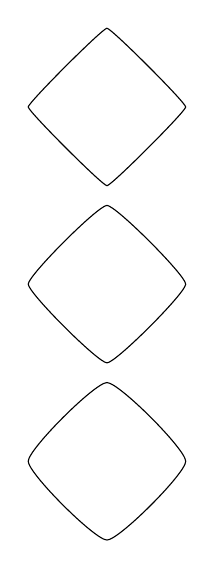
\begin{tikzpicture}[smooth cycle]
  \draw                 plot[tension=0.1]
    coordinates{(0,0) (1,1) (2,0) (1,-1)};
  \draw[yshift=-2.25cm] plot[tension=0.2]
    coordinates{(0,0) (1,1) (2,0) (1,-1)};
  \draw[yshift=-4.5cm]  plot[tension=0.275]
    coordinates{(0,0) (1,1) (2,0) (1,-1)};
\end{tikzpicture}
\end{codeexample}
  
  \itemoption{smooth cycle}
  This option causes the points on the path to be connected using a
  closed smooth curve. 

\begin{codeexample}[]
\tikz[scale=0.5]
  \draw plot[smooth cycle] coordinates{(0,0) (1,0) (2,1) (1,2)}
        plot               coordinates{(0,0) (1,0) (2,1) (1,2)} -- cycle;
\end{codeexample}

  \itemoption{ycomb}
  This option causes the |plot| command to interpret the plotting
  points differently. Instead of connecting them, for each point of
  the plot a straight line is added to the path from the $x$-axis to the point,
  resulting in a sort of ``comb'' or ``bar diagram.''

\begin{codeexample}[]
\tikz\draw[ultra thick] plot[ycomb,thin,mark=*] file{plots/pgfmanual-sine.table};
\end{codeexample}

\begin{codeexample}[]
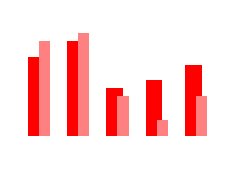
\begin{tikzpicture}[ycomb]
  \draw[color=red,line width=6pt]
    plot coordinates{(0,1) (.5,1.2) (1,.6) (1.5,.7) (2,.9)};
  \draw[color=red!50,line width=4pt,xshift=3pt]
    plot coordinates{(0,1.2) (.5,1.3) (1,.5) (1.5,.2) (2,.5)};
\end{tikzpicture}
\end{codeexample}

  \itemoption{xcomb}
  This option works like |ycomb| except that the bars are horizontal. 

\begin{codeexample}[]
\tikz \draw plot[xcomb,mark=x] coordinates{(1,0) (0.8,0.2) (0.6,0.4) (0.2,1)};
\end{codeexample}

  \itemoption{polar comb}
  This option causes a line from the origin to the point to be added
  to the path for each plot point.

\begin{codeexample}[]
\tikz \draw plot[polar comb,
     mark=pentagon*,mark options={fill=white,draw=red},mark size=4pt]
   coordinates {(0:1cm) (30:1.5cm) (160:.5cm) (250:2cm) (-60:.8cm)};
\end{codeexample}


  \itemoption{only marks}
  This option causes only marks to be shown; no path segments are
  added to the actual path. This can be useful for quickly adding some
  marks to a path.

\begin{codeexample}[]
\tikz \draw (0,0) sin (1,1) cos (2,0)
  plot[only marks,mark=x] coordinates{(0,0) (1,1) (2,0) (3,-1)};
\end{codeexample}
\end{itemize}



  

\subsection{The Scoping Operation}

When \tikzname\ encounters and opening or a closing brace (|{| or~|}|) at
some point where a path operation should come, it will open or close a
scope. All options that can be applied ``locally'' will be scoped
inside the scope. For example, if you apply a transformation like
|[xshift=1cm]| inside the scoped area, the shifting only applies to
the scope. On the other hand, a command like |color=red| does not have
any effect inside a scope since it can only be applied to the path as
a whole. 


\subsection{The Node Operation}

You can add nodes to a path using the |node| operation. Since this
operation is quite complex and since the nodes are not really part of
the path itself, there is a separate section dealing with nodes, see
Section~\ref{section-nodes}. 
